%% notes-tex/026-kinetics-thermodynamics/sections/3-thermodynamics.tex
%% [[experiments.026-metabolism-flux.kinetic-and-thermodynamic-parameter-datasets]]
%% https://github.com/Mjvolk3/torchcell/tree/main/notes-tex/026-kinetics-thermodynamics/sections/3-thermodynamics.tex

\section{Thermodynamics recomputed from eQuilibrator\secstatus{todo}}
\label{sec:thermo}

\subsection{Why the shipped table is a dead end\secstatus{todo}}

yeast-GEM 9.0.2 ships \texttt{model\_metDeltaG.csv} and \texttt{model\_rxnDeltaG.csv}, and
they are usable: 2{,}389 of 2{,}806 metabolites and 3{,}210 of 4{,}131 reactions carry a
value. They also close two doors. They are point values with no covariance, so the
correlated error term $\Delta_r G^{\circ,\mathrm{error}} = Qm$ that a thermodynamic flux
formulation calls for cannot be formed from them at all. And they exist only for this
model, so a table built on them transfers to no other organism.

Component contribution answers both at once. It decomposes a compound into groups, fits
group energies against the measured reaction corpus, and returns a formation energy
together with the covariance implied by that fit. Applied to a structure it works for any
organism, and for compounds no database has tabulated.

Reading the shipped files correctly is itself a trap worth recording. They use
\emph{two} missing-value conventions: most gaps are the sentinel $10^7$, but a further 51
metabolites and 120 reactions are the literal string \texttt{NaN}. Filtering only the
sentinel leaves the NaNs, which then propagate through every sum and produce NaN gradients
from what looks like a coverage of 87 percent.

\subsection{Resolution, and what it costs\secstatus{todo}}

Each metabolite is resolved by accession, MetaNetX first, then ChEBI, then KEGG, then
BiGG, with an InChI structure lookup as a fallback. Figure~\ref{fig:thermo-resolution}
shows where they land: MetaNetX carries almost all of it, and 332 metabolites resolve to
nothing.

\begin{figure}[H]
  \centering
  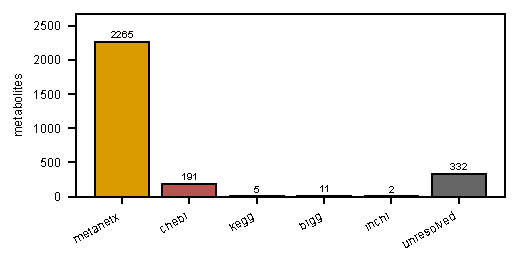
\includegraphics[width=0.62\textwidth]{figures/thermo_a_resolution.pdf}
  \caption[Metabolite resolution by identifier namespace]{Which identifier namespace
  resolved each of yeast-GEM's 2{,}806 metabolites to an eQuilibrator compound, in the
  order the resolver tries them. A metabolite counted under \texttt{chebi} is one whose
  MetaNetX identifier missed, so the bars are disjoint rather than nested. The 332
  unresolved are dominated by acyl-CoA isomers and the \texttt{biomass} pseudo-metabolite.
  Generated by \texttt{experiments/026-metabolism-flux/scripts/plot\_equilibrator\_thermo.py}.}
  \label{fig:thermo-resolution}
\end{figure}

The coverage cost is real and is stated rather than softened. Against the shipped table's
2{,}389 metabolites and 3{,}210 reactions, the recomputation covers 2{,}099 metabolites
(74.8 percent) and 1{,}755 reactions with every participant known (42.5 percent). Buying
uncertainty and organism-independence costs reaction coverage, because a reaction needs
\emph{all} of its participants resolved before it has an energy at all.

\subsection{The uncertainty, which is the point\secstatus{todo}}

Figure~\ref{fig:thermo-uncertainty} shows the standard error on the reactions whose energy
is estimable. Two facts sit inside it. Of 1{,}673 estimable reactions, 888 have a standard
error of exactly zero; those are transport reactions, where the same compound appears on
both sides of the membrane and its uncertainty cancels term by term. The remaining 785
carry a genuine standard error with a median of 2.30 kJ\,mol$^{-1}$ and a 95th percentile
of 6.01.

Estimability is a separate question from uncertainty and is easy to conflate. Component
contribution returns two sets of directions, one with finite variance and one with
infinite variance, the latter being directions the training corpus never determined.
Almost every individual compound has a nonzero infinite component, because an absolute
formation energy is defined only up to element conservation. Those directions cancel in a
mass-balanced reaction, which is exactly why the test must be applied to a reaction and
never to a compound in isolation. A reaction whose infinite component does not cancel has
an energy that is undefined rather than uncertain, and reporting it with a finite error bar
would be the most misleading thing this table could do, so it is masked instead.

\begin{figure}[H]
  \centering
  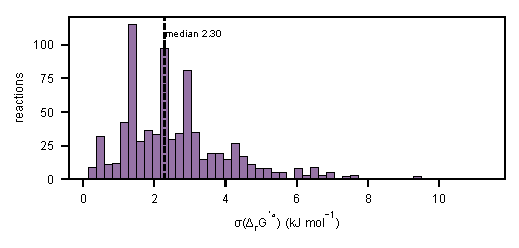
\includegraphics[width=0.62\textwidth]{figures/thermo_c_uncertainty.pdf}
  \caption[Reaction standard error from component contribution]{Standard error on
  $\Delta_r G'^\circ$ for the 785 estimable reactions whose uncertainty is nonzero, with
  the median marked. The 888 estimable reactions omitted here have a standard error of
  exactly zero because they are transport steps whose per-compound uncertainties cancel.
  The shipped table carries no uncertainty of any kind, so this quantity has no
  counterpart in it. Generated by
  \texttt{experiments/026-metabolism-flux/scripts/plot\_equilibrator\_thermo.py}.}
  \label{fig:thermo-uncertainty}
\end{figure}

\subsection{Agreement with the shipped table\secstatus{todo}}

Figure~\ref{fig:thermo-vs-shipped} compares the two tables on the 1{,}391 reactions both
cover, at a uniform pH 7.0 so that the comparison is between methods rather than between
pH assumptions.

The two classes of reaction must be read separately, and pooling them produces a
misleadingly good number. At a single uniform pH a transport reaction moves a species
between compartments with the same formation energy on both sides, so its energy here is
exactly zero by construction while the shipped table carries a nonzero value for it. Those
840 reactions form the horizontal band at zero. On the 551 chemical reactions, which is
where the two methods actually make comparable claims, the median absolute difference is
\textbf{10.11 kJ\,mol$^{-1}$}. Pooling all 1{,}391 gives 5.60, and that smaller number is
an artifact of the transport band rather than better agreement.

For scale, the shipped table disagrees with \emph{itself} by a comparable amount: the
reaction file and the reaction energies recomputed from its own metabolite file differ by a
median of 9.53 kJ\,mol$^{-1}$. So the two methods agree about as well as the shipped table
is internally consistent, which is the honest reading.

\begin{figure}[H]
  \centering
  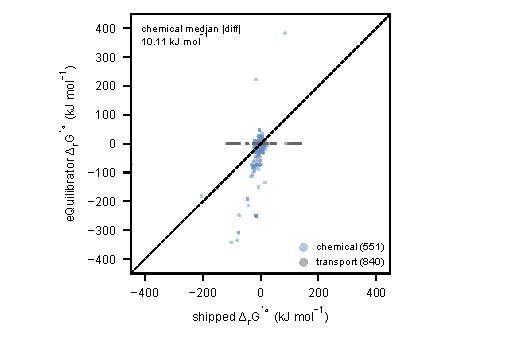
\includegraphics[width=0.62\textwidth]{figures/thermo_d_vs_shipped.pdf}
  \caption[eQuilibrator against the shipped reaction energies]{Reaction energies from the
  recomputation against the values yeast-GEM ships, on the 1{,}391 reactions both cover, at
  uniform pH 7.0, ionic strength 0.25 M and 303.15 K. Chemical reactions and transport
  reactions are separated because a transport step is exactly zero here by construction:
  at one pH the same species has the same formation energy in both compartments. The
  quoted median absolute difference is for the chemical subset. The dashed line is
  equality. Generated by
  \texttt{experiments/026-metabolism-flux/scripts/plot\_equilibrator\_thermo.py}.}
  \label{fig:thermo-vs-shipped}
\end{figure}

\subsection{Compartment pH is implemented and not trusted\secstatus{todo}}

Applying a per-compartment pH rather than a uniform one moves 1{,}309 of 1{,}755 covered
reactions, by a median of 42.2 kJ\,mol$^{-1}$ and by as much as 1{,}062
(Figure~\ref{fig:thermo-ph}). Shifts of that size are not physically plausible for single
reactions, so the uniform build is the artifact to use and the compartment build is
experimental. The pH table itself is textbook organellar values, recorded in the output as
\texttt{assumed}, not sourced from a mirrored paper.

The motivation for wanting it remains: a proton crossing a membrane between two pH values
is the entire driving force of a transport step, and computing every compartment at one pH
sets that force to zero by construction. Diagnosing the oversized shifts is open work.

\begin{figure}[H]
  \centering
  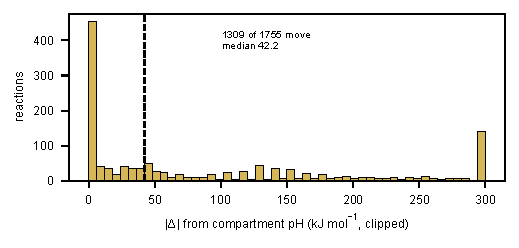
\includegraphics[width=0.62\textwidth]{figures/thermo_e_compartment_ph.pdf}
  \caption[Effect of compartment-specific pH]{Absolute change in $\Delta_r G'^\circ$ when
  each metabolite is transformed at its compartment's pH rather than at a uniform 7.0,
  over the reactions covered in both builds, clipped at 300 kJ\,mol$^{-1}$ for display.
  The median shift of 42.2 kJ\,mol$^{-1}$ is too large to be credible for ordinary
  reactions, which is why the uniform build is preferred. Generated by
  \texttt{experiments/026-metabolism-flux/scripts/plot\_equilibrator\_thermo.py}.}
  \label{fig:thermo-ph}
\end{figure}

\subsection{The correctness check\secstatus{todo}}

The table stores per-metabolite formation energies because that is what the flux layer
consumes, and reaction energies follow as $\sum_i S_{ij}\Delta_f G'^\circ_i$. That identity
is an assumption until tested: an error in the Legendre transform, in the compartment pH
assignment, or in a stoichiometric sign would each produce a table that looks entirely
reasonable and is wrong.

Pricing the same reactions both ways, by summing the table and by handing the resolved
compounds to eQuilibrator's own \texttt{standard\_dg\_prime}, agrees to a maximum absolute
difference of $9.1\times10^{-13}$ kJ\,mol$^{-1}$ over 40 single-compartment mass-balanced
reactions (Figure~\ref{fig:thermo-validation}). Only single-compartment reactions are used,
because a reaction spanning two compartments has no single pH and the API call would not be
answering the same question; only balanced ones, because an unbalanced reaction carries an
arbitrary offset.

As an absolute check that eQuilibrator is configured correctly before anything is compared
against it, four textbook reactions price at pH 7.2, ionic strength 0.25 M and 303.15 K as:
ATP hydrolysis $-28.93 \pm 0.30$, phosphoglucose isomerase $+2.66 \pm 0.38$, fumarase
$-3.43 \pm 0.28$ and triosephosphate isomerase $+5.61 \pm 0.55$ kJ\,mol$^{-1}$.

\begin{figure}[H]
  \centering
  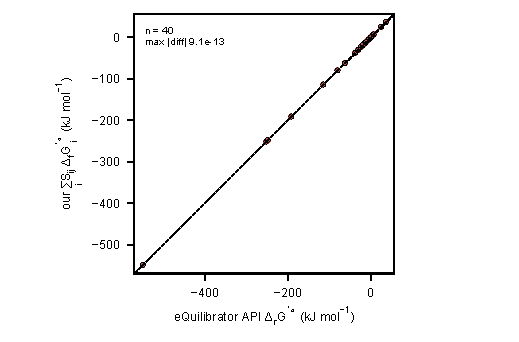
\includegraphics[width=0.62\textwidth]{figures/thermo_f_validation.pdf}
  \caption[Sum of formation energies against the eQuilibrator reaction call]{Reaction
  energies computed by summing our per-metabolite table against the same reactions priced
  directly by eQuilibrator's \texttt{standard\_dg\_prime}, over 40 randomly chosen
  single-compartment mass-balanced reactions. Maximum absolute difference
  $9.1\times10^{-13}$ kJ\,mol$^{-1}$, which is floating-point noise. This is a correctness
  check rather than a result: had the points left the diagonal, nothing else in this
  section would mean anything. Generated by
  \texttt{experiments/026-metabolism-flux/scripts/validate\_equilibrator\_thermo.py} and
  \texttt{plot\_equilibrator\_thermo.py}.}
  \label{fig:thermo-validation}
\end{figure}

\subsection{Where the method stops\secstatus{todo}}

The betaxanthin cassette is the test of the claim that this transfers to compounds no
database has tabulated. Of five intermediates, all five match their declared molecular
formula against a PubChem structure lookup, and two resolve to a formation energy:
L-DOPA at $-157.68$ with $\sigma = 4.30$, and dopaquinone at $-168.31$ with $\sigma = 7.54$
kJ\,mol$^{-1}$, both from structure alone with no identifier required.

The other three, cyclo-DOPA, betanidin and betalamic acid, are absent from the compound
cache, and the blocker is a \emph{commercial license rather than a method}. Creating a new
compound runs a group decomposition that needs pKa estimates, and eQuilibrator obtains
those from ChemAxon's \texttt{cxcalc}; without that license
\texttt{equilibrator\_assets} loads in read-only mode and refuses to create compounds. So
the generalization claim holds for structures the cache already knows and fails for
genuinely new ones. Closing the gap needs a pKa route that does not pass through ChemAxon,
not more plumbing.
